\section{Introducción}

Un aspecto muy importante dentro de la disciplina de desarrollo de software, tanto
a nivel de \textit{producto} como de \textit{proceso}, es la \textbf{calidad del
software}.
Ésta determina el grado en el que un producto satisface los requerimientos de sus usuarios
tanto internos como externos, y cómo les aporta valor a los mismos.

Se considera que un \textit{modelo de calidad} tiene el objetivo de describir, evaluar y/o
predecir la calidad de un componente \cite{Wagner2013}; y a lo largo de las últimas cuatro
décadas se han propuesto diferentes y diversos modelos \cite{Deissenboeck2009}.
Dentro de este conjunto de diversas propuestas podemos encontrar: modelos taxonómicos, como
lo es la familia de normas ISO/IEC 25000 \cite{ref}; modelos basados en métricas como el
índice de mantenibilidad (MI) \cite{ref}; modelos estocásticos, como los modelos de crecimiento
de confiabilidad (RGMs) \cite{ref}.

El problema existente con los tipos de modelos nombrados anteriormente viene dado por sus
diferentes propósitos, los cuales fueron clasificados por Deissenbock et al. \cite{Deissenboeck2009}
en tres categorías, y pueden verse en la figura \ref{DAPModels}.
La familia de normas ISO/IEC 25000 tiene como objetivo principal \textit{definir} lo que
corresponde a calidad en un sistema; mientras que un esquema orientado a métricas como MI
pretende \textit{evaluar} el nivel de calidad; mientras que los modelos de crecimiento de
confiabilidad se utilizan para \textit{predecir} la calidad.

Si bien los diferentes modelos se caracterizan por un objetivo particular, ya sea de
\textit{definición}, \textit{evaluación} o \textit{predicción}, éstos no son independientes,
debido a que es muy difícil evaluar calidad sin una propia definición de la misma, como también
es muy difícil predecir un determinado nivel de calidad sin saber cómo evaluarlo.

\begin{figure}
    \label{DAPModels}
    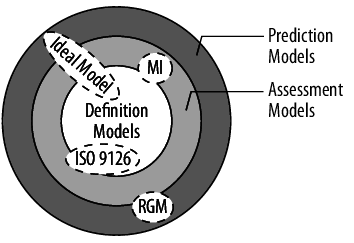
\includegraphics[width=12cm]{quality_metrics/dap_models.png}
    \centering
    \caption{Clasificación de Modelos de Calidad según su propósito.}
\end{figure}

AGREGAR ENGANCHE CON MANTENIBILIDAD.
Cuál sería?
Paper de Xi. Habla que la mantenibilidad es uno de los principales temas que atacan los diversos
estudios.

\section{Mantenibilidad}

\subsection{Definición}

Uno de de los modelos enfocados en la definición de calidad y sus diferentes aspectos
viene establecido por la familia de normas ISO/IEC 25000 \cite{ref}, 
la cual provee guías para obtener un producto de calidad, mediante la especificación 
de requisitos y características de calidad, así como la evaluación de las mismas.
Esta familia de normas está basada en dos normas anteriores (ISO/IEC 9126 \cite{ref}
e ISO/IEC 14598 \cite{ref}), y presenta cinco divisiones, las cuales se enfocan en diferentes
elementos y su proceso.

Particularmente, la norma ISO/IEC 25010, describe el modelo de calidad tanto para el producto
final como para el uso del mismo; definiendo así las características y subcaracterísticas
utilizadas en la evaluación de un elemento, siendo éstas:
\begin{inparaenum}[(1)]
    \item Adecuación funcional,
    \item Eficiencia de desempeño,
    \item Compatibilidad,
    \item Usabilidad,
    \item Fiabilidad,
    \item Seguridad,
    \item Mantenibilidad y
    \item Portabilidad.
\end{inparaenum}
Particularmente, la característica de \textbf{Mantenibilidad} representa la \textit{capacidad del
software para ser modificado de forma eficiente y efectiva, ya sea por motivos correctivos,
evolutivos o perfectivos}.

Así mismo, Mantenibilidad está compuesta por cinco subcaracterísticas:
\begin{inparaenum}[(a)]
    \item Modularidad,
    \item Reusabilidad,
    \item Analizabilidad,
    \item Capacidad para ser modificado \textit{(Modificabilidad)} y
    \item Capacidad para ser probado.
\end{inparaenum}
En el contexto de este trabajo, las subcaracterísticas de mayor interés corresponden
a la \textit{Analizabilidad} y la \textit{Modificabilidad}.
La \textbf{Analizabilidad} está asociada a la facilidad con la que se pueden diagnosticar problemas
o fallas en el software, identificar las partes/componentes de un sistema a modificar, y la
evaluación del impacto generado por los cambios.
Por otro lado, la \textbf{Modificabilidad} viene dada por la capacidad del producto para ser
modificado de forma efectiva y eficiente, sin introducir defectos o afectar la performance.

\subsection{Evaluación}

Así como la familia de normas ISO/IEC 25000 define un conjunto de características y
subcaracterísticas, también provee un listado básico de métricas para su medición.
Este listado no es exhaustivo, ya que se pueden emplear métricas no definidas por el
estándar, siempre y cuando se determine su correlación con alguna de las características
establecidas.
En la tabla \ref{Metrics} se listan las métricas definidas por el estándar, para la \textit{Mantenibilidad}
y sus subcaracterísticas.

\begin{figure}
    \label{Metrics}
    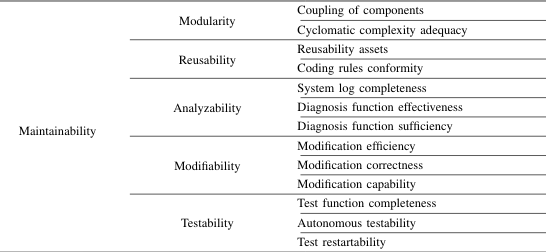
\includegraphics[width=12cm]{quality_metrics/quality_metrics.png}
    \centering
    \caption{Métricas para Mantenibilidad y su subcaracterísticas}
\end{figure}

Sin embargo, este conjunto de normas como otras existentes o anteriores sólo ofrecen una
guía muy abstracta sobre la definición de calidad de software, y no indican cómo lograr
que el software sea de calidad, ni cómo hacer una correcta medición \cite{Relf04}.
Al igual que los primeros modelos escritos a finales de la década de 1970, como los
propuestos por Boehm et al. \cite{Boehm1978} y McCall et al. \cite{McCall1977}, los cuales trataban
de definir la calidad de software como una descomposición jerárquica de características y
subcaracterísticas.

Por lo tanto, la investigación subsiguiente se enfocó principalmente en encontrar maneras de
cuantificar las propiedas definidas por los estudios anteriores.
Los trabajos de Dromey \cite{Dromey1995} y de Bansiya y Davis \cite{Bansiya2002}, son los más 
importantes ya que forman la base sobre la cual se construyeron los modelos más recientes, al 
describir cómo los atributos de alto nivel de calidad pueden medirse a partir de \textit{propiedades
de bajo nivel}, cuantificadas desde \textbf{métricas de software y análisis estático}.

Las contribuciones más significativas en el campo de la \textit{evaluación cuantitativa de la calidad},
basadas en el \textbf{análisis estático de código fuente} vienen dadas por el Modelo de Mantenibilidad 
SIG \cite{Heitlager2007}, junto con Quamoco tool chain \cite{Wagner2012}.

\subsubsection{Modelo de Mantenibilidad SIG}

Este modelo de evaluación de calidad \cite{Heitlager2007} permite determinar la mantenibilidad
de un proyecto de software, donde las características son descompuestas en un
conjunto de subcaracterísticas, y estas últimas en \textit{propiedades}.
Estas propiedades son cuantificables directamente desde el código fuente del producto, utilizando
análisis estático, permitiendo que a partir de estos valores junto con unos determinados umbrales,
cada propiedad reciba un \textit{perfil de calidad}.

Al poder cuantificar estas propiedades y obtener los perfiles, también se pueden agregar,
y de esta manera establecer un puntaje global de calidad del sistema.
Con el fin de mantener la objetividad en los umbrales para la evaluación de propiedades,
estos son obtenidos a través de benchmarking \cite{Alves2010}.

\subsubsection{Quamoco Tool Chain}

Similar al Modelo de Mantenibilidad SIG \cite{Heitlager2007}, Quamoco Tool Chain \cite{Wagner2012}
se basa en propiedades extraídas desde el código fuente a través de análisis estático del mismo,
con la diferencia de que permite a los interesados definir sus propios modelos jerárquicos
de calidad.

Quamoco define un meta-modelo, facilitando la creación de modelos más genéricos, en lugar de
estar restringidos a ciertos atributos de calidad como lo es la mantenibilidad, al introducir
el elementos que permiten cerrar la brecha entre medidas concretas y aspectos abstractos de
calidad.
Toma como base los atributos de calidad definidos en la norma ISO 25010, pero los refina
aplicando 200 factores y 600 mediciones para sistema Java y C\#.

\subsection{Predicción}

\textit{TBD}

\section{Impacto de los identificadores en Calidad de Software}

Tal como se establece en los diferentes estudios sobre los modelos de evaluación de
calidad \cite{XXX}, las métricas más utilizadas están relacionadas a la complejidad,
diseño y tamaño del código.
La particularidad de estas métricas, es que vienen dadas desde la extracción de
información a partir del código fuente.

Si bien el impacto que genera la baja calidad en el nombrado de los identificadores a la
comprensión de programas está razonablemente clara \cite{DeiBenbockPizka05,Lawrie2007,Lawrie2006},
se conoce relativamente poco sobre influencia que podría ejercer sobre la calidad del código fuente,
la calidad de los nombres de los indicadores per sé \cite{ButlerWemelingerYu10}.

"Existing research on source code readability focuses on the contribution the
components of source code make to readability" \cite{Buse2008}.

identificadores, y matching con convenciones vs. significado. \textbf{VER: YuSharp10}.

"Buse and Weimer \cite{Buse2008} developed a readability metric for Java derived from measurements 
of, among others, the number of parentheses and braces, line length, the number
of blank lines, and the number, frequency and length of identifiers.
Using machine learning, the readability metric was trained to agree with the judgement 
of human source code readers.
Buse and Weimer found a significant statistical relationship between the readability of 
methods and the presence of defects found by FindBugs in open source code bases. 
Although their work makes a link between readability and software quality, their notion
of readability ignores the quality of identifier names".

Se ignora el contenido semántico.

"The predictive probability associated with each relationship illustrates the utility
of the identifier flaws as light-weight classifiers for source code quality"
\cite{ButlerWemelingerYu10}.

\textbf{"a low-cost heuristic to identify potentially problematic regions of source code"}

"Software quality is not defined in terms of quality attributes but instead must be
inferred from characteristics that correlate to quality attributes and defect attributes.
One of these quality attributes is the readability of the software.
However, the software engineer, who is ultimately responsible for software quality,
is not supported well by their formal education, the software engineering culture, the
existence of useful tools and where these tools do exist by their limited up-take by industry.
Human cognitive limitations similarly frustrate the development of readable source code.
Software characteristics have been identified, which correlate well to source code readability.
One of these software characteristics, which have been supported by empirical research,
is the choice of identifier name".\cite{Relf04}

"A software characteristic that has the potential to improve software quality is the choice of
identifier name, and this is particularly so in large software systems.
identifier-naming sytle guidelines, supported by empirical evidence and generally accepted by
software professionals to direct towards improved source code readabiity are candidates for
automation by a tool.
Such an automated tool could make visibile aspects of software quality that are less keenly
perceived by the novice programmer and could assist in ther education along the path to
expert status"\cite{Relf04}.
